\documentclass[10pt,xcolor=table]{beamer}

% preamble.tex
\usepackage[T1,T2A]{fontenc}
\usepackage[utf8]{inputenc}
\usepackage[russian]{babel}
\usepackage{graphicx}
\usepackage{hyperref}
\usepackage{xcolor}
\usepackage{minted}

\usetheme{Madrid}
\usecolortheme{whale}

% Навигационные символы
\setbeamertemplate{navigation symbols}{}

\title{Анализ данных на F\#. Part 1}
\subtitle{FSharp.Data, XPlot}
\author{Никитин Артём 24Б44}
\date{\today}

\begin{document}

\maketitle

\begin{frame}[fragile]{FSharp.Data: Введение}
\inputminted{fsharp}{Code/fsharpData.fsx}
\vspace{0.5cm}
\begin{itemize}
    \item Ещё есть провайдеры для CSV, HTML, и XML
    \item Предоставляют простой доступ к структурированным данным
\end{itemize}
\vspace{0.3cm}
\end{frame}

\begin{frame}[fragile]{FSharp.Data: CSV}
\vspace{0.5cm}
\footnotesize{HLOC: High, Low, Open, Close — типичная структура финансовых данных}
\begin{center}
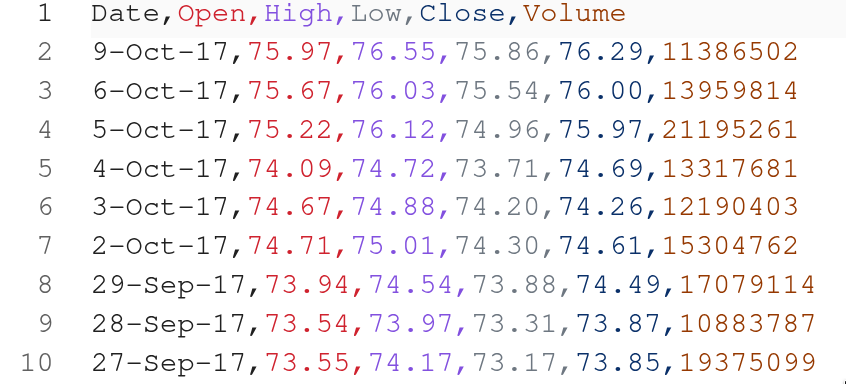
\includegraphics[width=\textwidth,height=0.85\textheight,keepaspectratio]{images/csvExample.png}
\end{center}
\vspace{0.3cm}
\end{frame}

\begin{frame}[fragile]{FSharp.Data: CSV Provider}
\inputminted{fsharp}{Code/CsvProviderp1.fsx}
\vspace{0.3cm}
\end{frame}

\begin{frame}[fragile]{FSharp.Data: CSV Provider}
\inputminted{fsharp}{Code/CsvProviderp2.fsx}
\vspace{0.3cm}
\end{frame}

\begin{frame}[fragile]{FSharp.Data: CSV Provider}
Что получилось:
\vspace{0.1cm}
\begin{minted}{console}
Last date: 10/9/2017 12:00:00 AM, Open: 75.97
HLOC: (76.55M, 75.86M, 75.97M, 76.29M)
HLOC: (76.03M, 75.54M, 75.67M, 76.00M)
HLOC: (76.12M, 74.96M, 75.22M, 75.97M)
HLOC: (74.72M, 73.71M, 74.09M, 74.69M)
HLOC: (74.88M, 74.20M, 74.67M, 74.26M)
HLOC: (75.01M, 74.30M, 74.71M, 74.61M)
HLOC: (74.54M, 73.88M, 73.94M, 74.49M)
HLOC: (73.97M, 73.31M, 73.54M, 73.87M)
HLOC: (74.17M, 73.17M, 73.55M, 73.85M)
HLOC: (73.81M, 72.99M, 73.67M, 73.26M)
\end{minted}
\vspace{0.3cm}
\end{frame}

\begin{frame}[fragile]{FSharp.Data: JSON Provider; Типизация}
\inputminted{fsharp}{Code/JsonProvider.fsx}
\vspace{0.3cm}
\begin{minted}{console}
F# Interactive:
type Simple = JsonProvider<...>
val simple: JsonProvider<...>.Root = {
  "name": "Tomas",
  "age": 4
}
val it: string = "Tomas"
\end{minted}
\vspace{0.3cm}
\end{frame}

\begin{frame}[fragile]{FSharp.Data: JSON Provider}
\inputminted{fsharp}{Code/Types.fsx}
\end{frame}

\begin{frame}[fragile]{FSharp.Data: JSON Provider; Работа с GitHub}
\inputminted{fsharp}{Code/GetIssue.fsx}
\vspace{0.3cm}
\begin{minted}{console}
#879 Bug when call request from Http module
#878 Header being considered as data row in HTMLProvider
\end{minted}
\vspace{0.3cm}
\end{frame}

\begin{frame}[fragile]{FSharp.Data: JSON Provider; Создание issue}
\inputminted{fsharp}{Code/CreateIssue.fsx}
\end{frame}

\begin{frame}[fragile]{XPlot}
\begin{itemize}
    \item На основе Plotly и Google Charts
    \item Plotly: Bar, (3D)Line, Area \dots
    \item Google Charts: Calendar, Geo, Pie \dots
    \item Network
\end{itemize}
\end{frame}

\begin{frame}[fragile]{XPlot: Bar Char}
\inputminted{fsharp}{Code/Basic.fsx}
\end{frame}

\begin{frame}[fragile]{XPlot: Bar Char}
\begin{center}
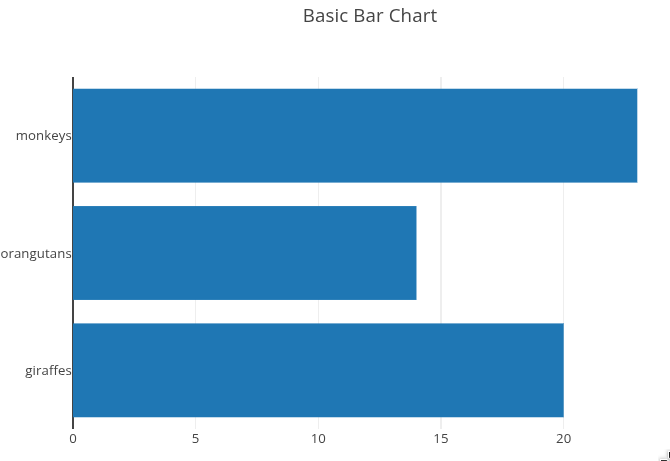
\includegraphics[width=\textwidth,height=0.85\textheight,keepaspectratio]{images/BasicBarChart.png}
\end{center}
\vspace{0.3cm}
\end{frame}

\begin{frame}[fragile]{XPlot: Grouped Bar Char}
\inputminted{fsharp}{Code/GroupedChar.fsx}
\end{frame}

\begin{frame}[fragile]{XPlot: Grouped Bar Char}
\begin{center}
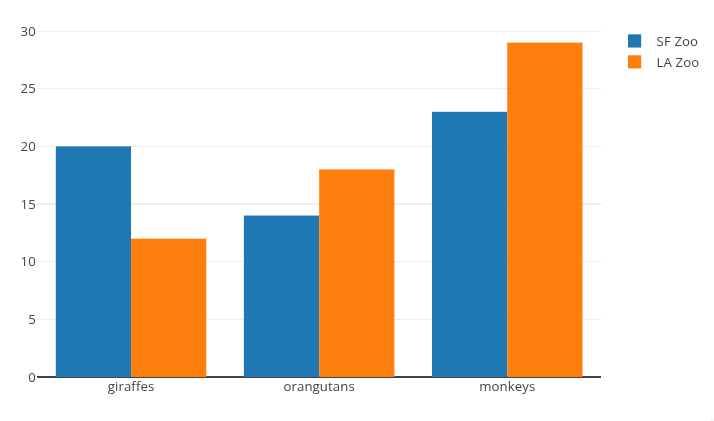
\includegraphics[width=\textwidth,height=0.85\textheight,keepaspectratio]{images/GBC.png}
\end{center}
\vspace{0.3cm}
\end{frame}

\end{document}